% ===================== sec_validation.tex =====================
% NOTE: sources: annotation_report.md, annotation_paper_paragraphs.tex, paper_tables/T5_annotation_agreement.tex, figure_manifest.md (Fig 12), claim_audit_report.md (X2, Check 4). The text follows Version B of the validation design: the annotators are language-model personas, and no claim of clinician validation is made. If real clinician annotations are obtained, this section must be rewritten.
% NOTE: the annotation files were committed first as ai_annotations/ and later renamed human_annotations/ (claim_audit_report.md, X2). State in the covering letter or the data statement that the set is simulated.
\section{Audit of the Labelling Pipeline}\label{sec:validation}

Every value in Section~\ref{sec:results} rests on one pipeline that extracts claims and classifies them (Section~\ref{sec:pipeline}). This section reports an audit of the labels that the pipeline assigns. The audit has a narrow scope. No clinician has annotated any part of the benchmark. The only independent annotation available is a set produced by six simulated annotators, and the audit therefore tests whether the pipeline agrees with an independent panel of language-model annotators. It does not test whether the pipeline agrees with the judgement of clinicians.

\subsection{Annotation set}\label{sec:val_set}
The set contains 720 generated texts, 180 for each modality. They are the responses of five models (Qwen2.5-VL, LLaVA-1.6, CheXagent, HuatuoGPT-Vision and LLaVA-Med) under the three conditions of the mitigation experiment (benchmark response, retrieval-augmented prompting and contrastive decoding), for 48 images, which are three for each combination of modality and query type. Each text was rated by six simulated annotators, which are a language model other than the pipeline judge prompted to act in six roles: a generalist, four modality specialists (radiology, dermatology, histopathology and ophthalmology) and an undergraduate student. Each annotator gave six scores on a scale from 0 to 5 (factual correctness, completeness, clinical safety, informativeness, clarity and overall quality) and flagged each of the seven hallucination classes as present or absent. The annotators are called simulated throughout, and the roles describe the instruction that each was given and not a qualification that any of them holds.
% NOTE: state which language model produced the annotations and the exact role prompts, or place them in the appendix.

Two properties of the set limit what it can show. First, the 720 texts rest on 48 images, with 15 texts for each image, so that the texts are clustered. Intervals in this section resample texts as if they were independent and are therefore too narrow. Second, \rad{the 12 radiology images are all the same file (Section~\ref{sec:data}), so that the radiology part of the set contains one radiograph}.

\subsection{Agreement among the simulated annotators}\label{sec:val_agree}
Table~\ref{tab:annotation} gives the agreement. The six annotators agree closely on the scores. The single-rater intraclass correlation, ICC(2,1), lies between \PH{0.829} for clinical safety and \PH{0.926} for clarity. The ICC for the mean of six raters is at least \PH{0.967}, and this value is high by construction in a fully crossed design with six raters. The agreement on the class flags is lower and depends on the class. The Fleiss $\kappa$ is \PH{0.70} for fabrication and \PH{0.78} for evasion, \PH{0.50} to \PH{0.51} for misclassification and severity distortion, and \PH{0.41}, \PH{0.36} and \PH{0.36} for omission, anatomical confusion and clinical reasoning error. Anatomical confusion was flagged for \PH{5\%} of the ratings, so that its $\kappa$ is unstable. Annotators in a specialist role did not agree more with the others on their own modality than on another one: for factual correctness the ICC of pairs formed by a specialist on the own modality and a non-specialist was \PH{0.853} [\PH{0.829}, \PH{0.872}], against \PH{0.864} [\PH{0.841}, \PH{0.881}] for pairs of specialists of other modalities.

These values describe the consistency of a set of language-model annotators and they should not be read as the reliability of human readers. The six annotators are driven by one generator and share its tendencies, so that agreement among them is expected to be higher than agreement among independent persons. The annotators also rated the texts severely, with a mean factual-correctness score of \PH{1.1} to \PH{2.2} on the scale of 5 depending on annotator and modality, and flagged at least one class for \PH{87\%} of the texts. Both properties lower $\kappa$ and raise raw agreement.

\begin{table}[t]
\centering
\small
\begin{tabular}{lcccc}
\toprule
Score (0--5) & ICC(2,1) [95\% CI] & ICC(2,k) & Alpha & QWK \\
\midrule
factual correctness & 0.860 [0.842, 0.877] & 0.974 & 0.860 & 0.845 \\
completeness & 0.863 [0.845, 0.881] & 0.974 & 0.863 & 0.842 \\
clinical safety & 0.829 [0.809, 0.847] & 0.967 & 0.829 & 0.812 \\
informativeness & 0.858 [0.840, 0.874] & 0.973 & 0.857 & 0.840 \\
clarity & 0.926 [0.914, 0.937] & 0.987 & 0.926 & 0.915 \\
overall & 0.877 [0.860, 0.892] & 0.977 & 0.877 & 0.862 \\
\bottomrule
\end{tabular}
\par\medskip
\small
\begin{tabular}{lcccc}
\toprule
Hallucination class & Prevalence & Fleiss $\kappa$ [95\% CI] & Judge vs. majority $\kappa$ [95\% CI] & Judge F1 \\
\midrule
Fabrication & 0.59 & 0.70 [0.66, 0.73] & 0.40 [0.34, 0.47] & 0.74 \\
Omission & 0.26 & 0.41 [0.37, 0.44] & 0.18 [0.12, 0.24] & 0.51 \\
Misclassification & 0.35 & 0.50 [0.46, 0.54] & 0.04 [0.00, 0.08] & 0.10 \\
Severity distortion & 0.40 & 0.51 [0.48, 0.55] & 0.11 [0.05, 0.17] & 0.30 \\
Anatomical confusion$^{a}$ & 0.05 & 0.36 [0.28, 0.43] & -0.01 [-0.02, -0.01] & undef. \\
Evasion & 0.20 & 0.78 [0.74, 0.81] & -0.06 [-0.09, -0.03] & 0.01 \\
Clinical reasoning error & 0.10 & 0.36 [0.30, 0.42] & 0.15 [0.08, 0.23] & 0.25 \\
\bottomrule
\end{tabular}
\caption{Agreement among six \emph{simulated (AI-persona) annotators} on 720 items (48 distinct images), and between the LLM judge and the annotator majority. No clinician annotations are included. Intervals are 95\% item-level bootstrap CIs and are optimistic because items share images; $^{a}$ rare class, $\kappa$ unstable.}
\label{tab:annotation}
\end{table}


\begin{figure*}[t]
  \centering
  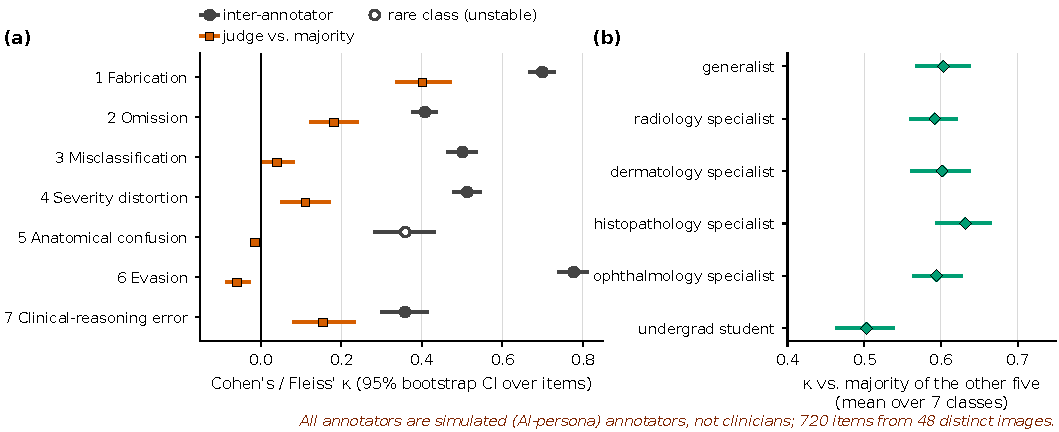
\includegraphics[width=\textwidth]{paper_figures/fig12_annotation_agreement.pdf}
  \caption{(a) Agreement per hallucination class among the six simulated annotators (Fleiss $\kappa$) and between the language-model judge and their majority label (Cohen $\kappa$), for 720 texts from 48 images. (b) Mean $\kappa$ of each annotator with the majority of the other five. Bars are 95\% bootstrap intervals over texts (2{,}000 resamples), which are too narrow because texts share images. No clinician annotation is included.}
  \label{fig:annotation}
\end{figure*}

\subsection{Agreement of the pipeline with the annotator majority}\label{sec:val_judge}
The pipeline was compared with the majority of the simulated annotators. A class is positive for a text if at least four of the six annotators flag it, and a tie of three against three is resolved by the annotator in the role of specialist for the modality of the text. The annotators flag classes for a whole text, so the comparison is made at the level of the text. The claim-level output of the pipeline is aggregated by marking a class as present if any claim is assigned to it, and the omissions of Layer 1 are counted in the omission class, as in the definition of the \SMHR{}. Three of the 720 texts have no usable pipeline label, which leaves 717.

\paragraph{Any hallucination.} The combined label of the pipeline, positive when any class is present, reached a precision of \PH{0.888}, a recall of \PH{0.901} and an $F_1$ of \PH{0.895} [\PH{0.877}, \PH{0.912}] against the majority label. The threshold of 0.90 set in the study protocol was therefore not met at the point estimate, and the interval spans it. The thresholds set for the layers taken separately (0.95 for Layer 1 and 0.90 for Layer 2) were not met either; the layer-wise comparisons use the label for all classes and are indicative. By modality, the $F_1$ of the combined label was \PH{0.971} [\PH{0.950}, \PH{0.986}] in radiography \rad{(one radiograph)}, \PH{0.841} [\PH{0.795}, \PH{0.886}] in dermoscopy, \PH{0.903} [\PH{0.867}, \PH{0.936}] in histopathology and \PH{0.848} [\PH{0.803}, \PH{0.888}] in fundus photography.

This $F_1$ is not good evidence of discrimination. The annotators flagged at least one class for \PH{626} of the \PH{717} texts, which is \PH{87\%}, and a rule that flags every text would reach a precision of \PH{0.873}, a recall of 1 and an $F_1$ of \PH{0.932}, higher than the value of the pipeline. The Cohen $\kappa$ of the combined label with the majority is \PH{0.126}, which indicates only slight agreement beyond chance. At this prevalence the $F_1$ for the presence of any hallucination cannot separate a labelling pipeline from a rule that always reports a hallucination, and the audit does not support a claim of validation at this level.

\paragraph{Individual classes.} Class-level agreement is weaker (Table~\ref{tab:annotation} and Figure~\ref{fig:annotation}). Fabrication is the class that the pipeline reproduces best, with a precision of \PH{0.767}, a recall of \PH{0.714}, an $F_1$ of \PH{0.74} and a $\kappa$ of \PH{0.40} [\PH{0.34}, \PH{0.47}]. Omission is over-called, with a precision of \PH{0.385} and a recall of \PH{0.751} ($F_1$ \PH{0.51}, $\kappa$ \PH{0.18}). The pipeline rarely assigns misclassification, severity distortion or evasion, which the annotators flag often; its recall for them is \PH{0.053}, \PH{0.206} and \PH{0.007}. For anatomical confusion, the pipeline found none of the \PH{30} texts that the majority flagged. For clinical reasoning error the pipeline flags \PH{153} texts against \PH{51} for the majority, with a precision of \PH{0.163}. The class that the pipeline regards as the most severe in a text agrees with that of the majority for \PH{55\%} of the texts.

Two differences between the methods qualify these figures. The annotators judge a text as a whole against their own reading of the case, while the pipeline compares claims with the reference labels, which record only a subset of the findings in an image, so that the two do not define omission or evasion in the same way. Differences between them therefore do not show which of the two is closer to the intended meaning of a class. The values nevertheless establish that the class-specific labels of the pipeline cannot be described as validated, and the class composition reported in Section~\ref{subsec:res_modality} is descriptive only.

\subsection{Relation to the item-level \SMHR{}}\label{sec:val_smhr}
A weaker check does not depend on the class flags. For each text with at least one claim, the mean factual-correctness score of the annotators was correlated with the \SMHR{} of the text. The Spearman correlation was \PH{$-0.31$} [\PH{$-0.38$}, \PH{$-0.23$}] for \PH{682} texts, in the expected direction and of moderate size. It was \PH{$-0.47$} in dermoscopy, \PH{$-0.34$} in fundus photography and \PH{$-0.20$} in radiography \rad{}, and the interval included zero in histopathology (\PH{$-0.08$} [\PH{$-0.24$}, \PH{0.08}]). A moderate correlation is the size that is expected between a holistic rating and a ratio of weighted claims. At the level of the model, the rank correlation between the mean factual-correctness score of each annotator and the \SMHR{} was \PH{$-0.7$} for the five models, which is moderate and rests on five points.

\subsection{What the audit supports}\label{sec:val_summary}
The audit supports three statements. The pipeline agrees moderately with an independent panel of language-model annotators for the presence of fabrication, and weakly for most other classes. Its text-level \SMHR{} is moderately and negatively related to the factual-correctness ratings of the panel. The ranking of the models and the comparison of domain-adapted and general-purpose models do not depend on the class weights within the ranges tested (Section~\ref{subsec:res_robust}). The audit does not support the statements that clinicians would agree with the labels, that the class weights reflect clinical harm, or that the class-specific labels are valid. Agreement with an independent language-model panel is weaker evidence than agreement with clinicians, because the panel and the judge may share errors of a kind that readers of images would not make.
